% CVPR 2024 Paper Template; see https://github.com/cvpr-org/author-kit

\documentclass[10pt,twocolumn,letterpaper]{article}

%%%%%%%%% PAPER TYPE  - PLEASE UPDATE FOR FINAL VERSION
\usepackage{cvpr}              % To produce the CAMERA-READY version
% \usepackage[review]{cvpr}      % To produce the REVIEW version
% \usepackage[pagenumbers]{cvpr} % To force page numbers, e.g. for an arXiv version

\usepackage[accsupp]{axessibility} % Improves PDF readability for those with visual impairments.

% Import additional packages in the preamble file, before hyperref
\usepackage{graphicx}
\usepackage{color}
\usepackage{symbol}
\usepackage{placeins}
\usepackage{booktabs}
\usepackage{soul}
\usepackage{nicefrac}
\usepackage{wrapfig, tikz}
\usepackage{amsmath,amsfonts,bm,xspace}
\usepackage{bbm}
\usepackage{color}
\usepackage{enumitem, multirow}
\usepackage{fontawesome5}
\usepackage[many]{tcolorbox}
\usepackage{colortbl}


% It is strongly recommended to use hyperref, especially for the review version.
% hyperref with option pagebackref eases the reviewers' job.
% Please disable hyperref *only* if you encounter grave issues, 
% e.g. with the file validation for the camera-ready version.
%
% If you comment hyperref and then uncomment it, you should delete *.aux before re-running LaTeX.
% (Or just hit 'q' on the first LaTeX run, let it finish, and you should be clear).
\usepackage[dvipsnames]{xcolor}
\definecolor{cvprblue}{rgb}{0.21,0.49,0.74}
\usepackage[pagebackref,breaklinks,colorlinks,citecolor=cvprblue]{hyperref}
\usepackage{float}
\usepackage{marvosym}
\usepackage{amsmath}

%%%%%%%%% PAPER ID  - PLEASE UPDATE
% \def\paperID{2291} % *** Enter the Paper ID here
% \def\confName{CVPR}
% \def\confYear{2024}

%%%%%%%%% TITLE - PLEASE UPDATE
\title{From Parts to Whole: A Unified Reference Framework for Controllable Human Image Generation}

%%%%%%%%% AUTHORS - PLEASE UPDATE
\author{
    {
        Zehuan Huang\footnotemark[1] \quad Hongxing Fan\footnotemark[1] \quad Lipeng Wang\footnotemark[1] \quad Lu Sheng\footnotemark[2]
    }\\
    {Beihang University} \\
    {\tt\small \{huangzehuan, fanhongxing, wanglipeng, lsheng\}@buaa.edu.cn}\\
    {\small\url{https://huanngzh.github.io/Parts2Whole/}}
}

\begin{document}

\twocolumn[\maketitle\vspace{-2.5em}\begin{figure}[!ht]
    \begin{minipage}{0.65\textwidth}
        \centering
        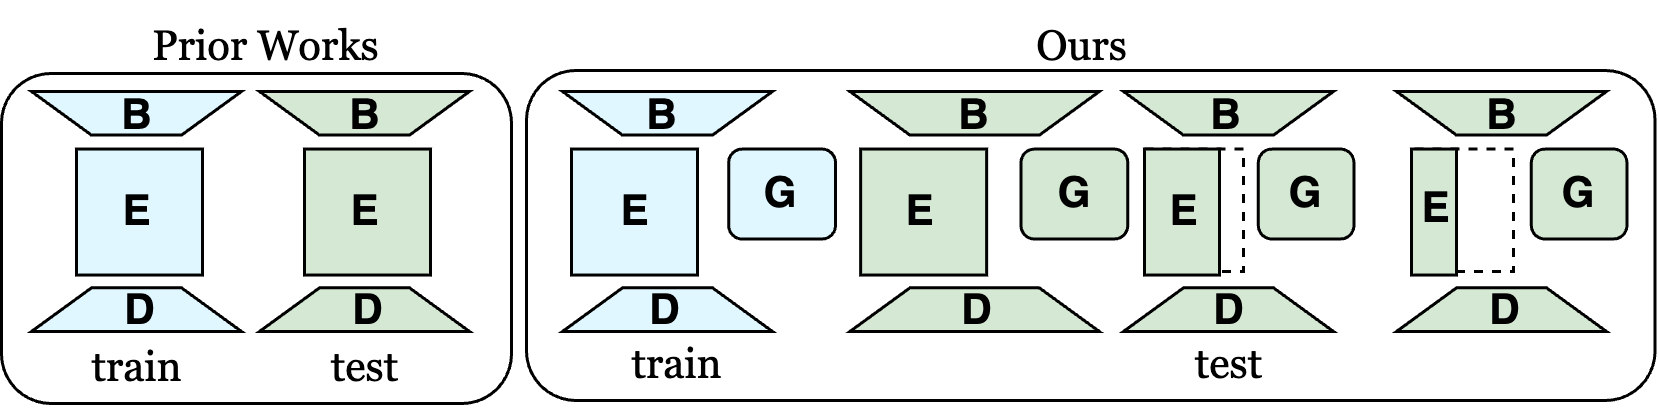
\includegraphics[width=\textwidth]{figures/images/teaser.png}
      \caption{\textbf{Comparison to prior works.} Instead of conventional M2F-style architecture that provides ``one-size-fits-all'' solution, our method \ours focuses on training such models in order to directly run at various resource encoder depths by leveraging a gating function. Here, \textbf{B}, \textbf{E}, \textbf{D}, and \textbf{G} denote the backbone, encoder, decoder, and (our proposed) gating network, respectively.} %
      \label{fig:teaser_a}
    \end{minipage}%
    \hfill
    \begin{minipage}{0.3\textwidth}
        \centering
        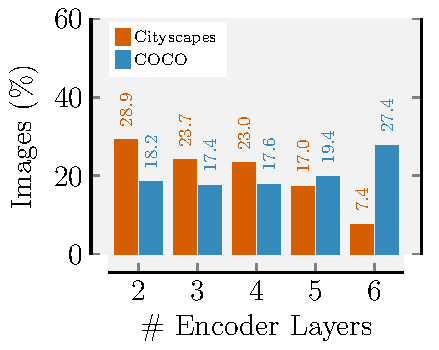
\includegraphics[width=\textwidth]{figures/images/image_vs_layer_barplot.pdf}
        \caption{Histogram of images achieving best panoptic segmentation by number of encoder layers.}
        \label{fig:teaser_b}
    \end{minipage}
    
\end{figure}\bigbreak]

\renewcommand{\thefootnote}{\fnsymbol{footnote}}
\footnotetext[1]{Equal Contribution.}
\footnotetext[2]{Corresponding author.}


\begin{abstract}
Inverse graphics -- the task of \textit{inverting} an image into physical variables that, when rendered, enable reproduction of the observed scene -- is a fundamental challenge in computer vision and graphics.
Disentangling an image into its constituent elements, such as the shape, color, and material properties of the objects of the 3D scene that produced it, requires a comprehensive understanding of the environment.
This requirement limits the ability of existing carefully engineered approaches to generalize across domains.
Inspired by the zero-shot ability of large language models (LLMs) to generalize to novel contexts, we investigate the possibility of leveraging the broad world knowledge encoded in such models in solving inverse-graphics problems.
To this end, we propose the Inverse-Graphics Large Language Model (\mbox{\textit{IG-LLM}}), an inverse-graphics framework centered around an LLM, that autoregressively decodes a visual embedding into a structured, compositional 3D-scene representation.
We incorporate a frozen pre-trained visual encoder and a continuous numeric head to enable end-to-end training.
Through our investigation, we demonstrate the potential of LLMs to facilitate inverse graphics through next-token prediction, without the use of image-space supervision.
Our analysis opens up new possibilities for precise spatial reasoning about images that exploit the visual knowledge of LLMs.
We will release our code and data to ensure the reproducibility of our investigation and to facilitate future research at \hbox{\url{https://ig-llm.is.tue.mpg.de/}}
\end{abstract}
\section{Introduction}

\label{sec:intro}

Reconstructing a 3D scene from video is one of the most fundamental problems in vision and has been studied for over five decades.
Today, essentially all state-of-the-art approaches are built on top of Structure-from-Motion (SfM) methods like COLMAP~\cite{schonberger2016structure}. These approaches extract sparse correspondences across frames, match them, discard outliers, and then optimize the correspondences' 3D positions alongside the camera parameters by minimizing reprojection error~\cite{schonberger2016structure}.

This framework has delivered excellent results which underlie many present-day vision applications, and so it is unsurprising that SfM systems have remained largely unchanged in the age of deep learning, save for deep-learning-based correspondence matching \cite{sarlin2020superglue,lindenberger2023lightglue,sarlin2021pixloc,detone2018superpoint}.

However, conventional SfM has a major limitation: it is not differentiable with respect to its free variables (camera poses, camera intrinsics, and per-pixel depths).
This means that SfM acts as an isolated pre-processing step that cannot be embedded into end-to-end deep learning pipelines. 
A differentiable, self-supervised SfM method would enable neural networks to be trained self-supervised on internet-scale data for a broad class of multi-view geometry problems.
This would pave the way for deep-learning based 3D reconstruction and scene understanding.

\begin{figure*}[t]
    \centering
    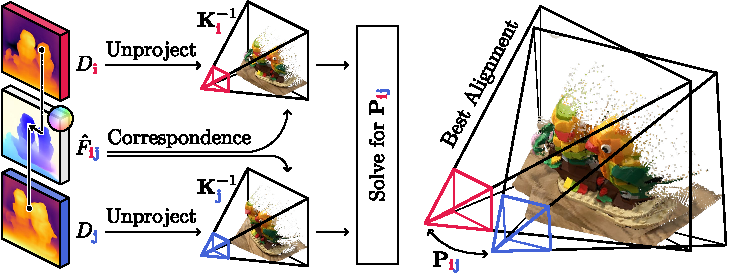
\includegraphics[width=\linewidth,]{figures/procrustes/fig_procrustes_pdf_small.pdf}
    \vspace{-12pt}
    \caption{We solve for the relative poses between consecutive frames using their depth maps, camera intrinsics, and optical flow. To do so, we first unproject their depth maps, then solve for the pose that best aligns the resulting point clouds.}
    \label{fig:procrustes}
    \vspace{-15pt}
\end{figure*}

In this paper, we present FlowMap, a differentiable and surprisingly simple camera and geometry estimation method whose outputs enable photorealistic novel view synthesis. 
FlowMap directly minimizes the difference between optical flow that is induced by a camera moving through a static 3D scene and pre-computed correspondences in the form of off-the-shelf point tracks and optical flow.
Since FlowMap is end-to-end differentiable, it can naturally be embedded in any deep learning pipeline.
Its loss is minimized only via gradient descent, leading to high-quality camera poses, camera intrinsics, and per-pixel depth.
Unlike conventional SfM, which outputs sparse 3D points that are each constrained by several views, FlowMap outputs dense per-frame depth estimates.
This is a critical advantage in downstream novel view synthesis and robotics tasks.
Unlike prior attempts at gradient-based optimization of cameras and 3D geometry~\cite{lin2021barf,nerf--,bian2022nopenerf}, we do not treat depth, intrinsics, and camera poses as free variables.
Rather, we introduce differentiable feed-forward estimates of each one: depth is parameterized via a neural network, pose is parameterized as the solution to a least-squares problem involving depth and flow, and camera intrinsics are parameterized using a differentiable selection based on optical flow consistency.
In other words, FlowMap solves SfM by learning the depth network's parameters; camera poses and intrinsics are computed via analytical feed-forward modules without free parameters of their own.
We show that this uniquely enables high-quality SfM via gradient descent while making FlowMap compatible with standard deep-learning pipelines.
Unlike recent radiance-field bundle-adjustment baselines~\cite{bian2022nopenerf,lin2021barf}, FlowMap does not use differentiable volume rendering, and so it is significantly faster to run, generally reconstructing an object-centric $360^\circ$ scan in less than 10 minutes.

Through extensive ablation studies, we show that each of FlowMap's design choices is necessary.
On popular, real-world novel view synthesis datasets (Tanks \& Temples, Mip-NeRF 360, CO3D, and LLFF), we demonstrate that FlowMap enables photo-realistic novel view synthesis up to full $360^\circ$ trajectories using Gaussian Splatting~\cite{kerbl20233d}. 
Gaussian Splats obtained from FlowMap reconstructions far outperform the state-of-the-art gradient-based bundle-adjustment method, NoPeNeRF~\cite{bian2022nopenerf}, and those obtained using the SLAM algorithm DROID-SLAM~\cite{teed2021droid}, even though both baselines require ground-truth intrinsics.
Gaussian Splats obtained from FlowMap are on par with those obtained from COLMAP~\cite{schonberger2016structure}, even though FlowMap only leverages gradient descent, is fully differentiable, and represents a complete departure from conventional SfM techniques.

\section{Related Work}

\cparagraph{Text-to-Image Generation.}
In recent years, text-to-image generation has made remarkable progress, particularly with the development of diffusion models~\cite{ramesh2022dalle2, nichol2022glide, rombach2022ldm, saharia2022imagen, dhariwal2021diffusionbeatgans, ho2020ddpm, podell2023sdxl, huang2023epidiff} and auto-regressive
models~\cite{chang2023muse, yu2022scalingauto, tian2024var}, which have propelled text-to-image generation to large-scale commercialization. Since DALLE2~\cite{ramesh2022dalle2}, Stable Diffusion~\cite{rombach2022ldm} and Imagen~\cite{saharia2022imagen} employ diffusion models as generative models and train the models on large datasets, text-to-image synthesis ability has been significantly enhanced. More recently, Stable Diffusion XL~\cite{podell2023sdxl}, a two-stage cascade diffusion model, has greatly improved the generation of high-frequency details and overall image color, taking aesthetic appeal to a higher level. However, these existing methods are limited to generating images solely from text prompts, and they do not meet the demand for producing customized images with the preservation of appearance.

\cparagraph{Controllable Image Generation.}
Given the robust generative capabilities of image diffusion models, a series of research~\cite{zhang2023controlnet, mou2023t2iadapter, qin2023unicontrol, ruiz2023dreambooth, hu2021lora, ye2023ipadapter, chen2023anydoor, zhang2024ssrencoder} attempts to explore the controllability of image generation, enabling image synthesis guided by multi-modal conditions. Some work~\cite{zhang2023controlnet, mou2023t2iadapter, jiang2023scedit, qin2023unicontrol, zhao2024unicontrolnet, hu2023cocktail} focuses on introducing structural signals such as edges, depth maps, and segmentation maps, to control the spatial structure of generated images. Another group of work~\cite{ruiz2023dreambooth, hu2021lora, gal2022textualinversion, ye2023ipadapter, chen2023anydoor} uses appearance conditions to guide image generation, aiming to generate images aligning with specific concepts like identity and style, known as subject-driven image generation. The methods generally fall into two categories: those requiring test-time fine-tuning and those that do not. Test-time fine-tuning methods~\cite{ruiz2023dreambooth, hu2021lora, gal2022textualinversion, kumari2023customdiffusion, liu2023cones} often optimizes additional text embedding, parameter residuals or direct fine-tune the whole model to fit the specified subject. Although these methods have achieved impressive results, they cost about half an hour to achieve satisfactory results. Fine-tuning-free methods~\cite{shi2023instantbooth, ye2023ipadapter, chen2023anydoor, zhang2024ssrencoder, ma2023subjectdiffusion, gal2023encoderdiff, wei2023elite} typically train an additional encoding network to encode the reference image into embeddings or image prompts. However, due to the loss of spatial representations when encoding the reference images into one or a few tokens, they struggle to preserve appearance details.

\cparagraph{Controllable Human Image Generation.}
In this paper, we mainly focus on controllable human image generation and aim to synthesize human images aligning with specific text prompts, pose signals, and various parts of human appearance. Text2Human~\cite{jiang2022text2human} generates full-body human images using detailed descriptions about the textures of clothes, but is limited by the coarse-grained textual condition. Test-time fine-tuning methods~\cite{ruiz2023dreambooth,hu2021lora,kumari2023customdiffusion} produce satisfactory results, but when it comes to customizing portraits using multiple parts of human appearance, they take much more time to fit each aspect. Recently, methods like IP-Adapter-FaceID~\cite{ye2023ipadapter}, FastComposer~\cite{xiao2023fastcomposer}, PhotoMaker~\cite{li2023photomaker}, and InstantID~\cite{wang2024instantid} show promising results on zero-shot human image personalization. They encode the reference face to one or several tokens as conditions to generate customized images. With the addition of adaptable structural control networks~\cite{zhang2023controlnet, mou2023t2iadapter}, these methods can generate portraits aligned with specified poses and human identities. However, they usually fail to maintain the details of human identities and utilize all the information from a single image, resulting in ambiguous subject representation. These make it difficult to apply these schemes to precisely generation conditioned on multiple parts of the human appearance. In contrast, our Parts2Whole is both generalizable and efficient, and precisely retains details in multiple parts of human appearance.
\section{Method}

In this section, we detail our STAR-MT method and the domain adaptation benchmark. The overall scheme of the proposed solution is illustrated in Fig.\ref{fig:SFVOD}. 

\subsection{Mean-teacher for domain adaptive VOD}
 In developing our method, we leverage the advanced unsupervised domain adaptation strategies found in the mean-teacher self-training approach \cite{tarvainen2017mean}. We introduce the implementation of this method in this paradigm.
 
 As a class of student-teacher training approach, the mean-teacher method keeps two identical networks: the student network and the teacher network. They are initialized by the weights trained on the source domain. During training, the weights of the teacher model are fixed, while the student model is trained with the supervision signal from the prediction output and features generated from the teacher model. On the other hand, the teacher model takes the exponential moving average (EMA) of consecutive student models for its parameter update:
\begin{equation}
    \theta_{\mathcal{T}}^{t} \leftarrow \alpha \theta_{\mathcal{T}}^{t-1} + (1-\alpha) \theta_{\mathcal{S}}^{t-1},
\end{equation}
where the $\theta_{\mathcal{T}}$ and $\theta_{\mathcal{S}}$ denote the weights of teacher and student models, $t$ denotes the training iteration, and $\alpha \in (0,1)$ is the momentum coefficient which is usually set close to 1 for a smooth temporal ensemble \cite{cao2023contrastive}.
 
\subsection{Spatial-Temporal Alternate Refinement}
YOLOV utilized the pre-trained backbone of YOLOX as its frame-wise feature extractor, followed by feature selection and affinity measurement that identifies features from the same object among frames to guide temporal aggregation. However, training the spatial backbone and temporal aggregation module simultaneously on the video object detection dataset is suboptimal because they require different training schemes. Hence, we propose to adapt the YOLOV in a two-stage alternate optimization manner, consisting of the temporal refinement stage (TRS) and spatial refinement stage (SRS).

\subsubsection{Temporal Refinement Stage (TRS).}
In the TRS, the entire teacher model, including the frame-wise backbone and temporal aggregation module, is updated via EMA. In the beginning, both teacher and student models are initialized the same.
Like a typical mean-teacher-based algorithm, the same image sequences with different augmentations are fed into those models. The teacher model processes the weakly augmented images, and the heavily augmented images are fed into the student model. Moreover, we randomly mask out $r\%$ frames and enforce the student model to produce the same output with fewer frames than the teacher model. This masking mechanism can supposedly enhance the generalization capability of temporal aggregation. The student model is trained by aligning frame-wise features and soft pseudo labels with the features and predictions of the teacher model. The loss in this stage is defined as:
\begin{equation}
    \mathcal{L} = \mathcal{L}_{MSE}(f_{\mathcal{T}}, f_{\mathcal{S}}) + \mathcal{L}_{BCE}(y_{\mathcal{T}}^{cls}, y_{\mathcal{S}}^{cls}),
\end{equation}
where the first term is the mean square error between the feature maps $f_{\mathcal{T}}$ and $f_{\mathcal{S}}$, produced by the backbone module of the teacher and student models, respectively. The term $\mathcal{L}_{BCE}$ denotes the binary cross entropy loss. $y_{\mathcal{T}}^{cls}$ refers to the top-$k$ classification prediction after the temporal aggregation of the teacher model, and $y_{\mathcal{S}}^{cls}$ refers to that of the student model. $k$ is the number of proposals in the feature selection module before the temporal aggregation. We set $k=30$ following the default setting of YOLOV. We do not particularly compute the loss of objectiveness and bounding box prediction because they are unchanged in the temporal aggregation module. 


\subsubsection{Spatial Refinement Stage (SRS).} 
TAM consists of two key components: a Feature Selection Module, which selects high-quality prediction proposals, and a Feature Aggregation Module, which fuses these proposals across multiple frames. However, due to the inconsistency between the training pipelines of the single-frame detection head (backbone) and the TAM, the TRS, which mostly follows the training setting of the TAM, may lead to suboptimal adaptation on the backbone side. Recognizing that the TAM can reliably improve prediction quality, we propose using the output class score of YOLOV, instead of YOLOX, in the teacher model as higher-quality pseudo labels to guide the fine-tuning of the detection head of YOLOX in the student model. In the SRS, only the backbone of the teacher model is updated via EMA, ensuring that the adaptation focuses on the spatial feature extraction process while leveraging the enhanced temporal information from the TAM. The loss is given as follows:
\begin{equation}
    \mathcal{L} = \mathcal{L}_{MSE}(f_{\mathcal{T}}, f_{\mathcal{S}}) + \mathcal{L}_{BCE}(y_{\mathcal{T}}^{cls}, y_{\mathcal{S}}^{cls}) + \gamma \mathcal{L}_{cls},
\end{equation}

\noindent where $\gamma$ is the weighting factor. The new loss term $\mathcal{L}_{cls}$ is the certainty-aware binary cross entropy loss between the filtered class score from the teacher and student model:
\begin{equation}
\begin{aligned}
    \mathcal{L}_{cls}  = -\frac{1}{N}\sum_{i}^{N} p^{i}_{\mathcal{S}} \Big[ \frac{1}{n_{c}} & \sum_{c}^{n_c}  \left( s_{\mathcal{T}}^{i,c} \log(s_{\mathcal{S}}^{i,c}) \right. \\
    & \left.  +(1-s_{\mathcal{T}}^{i,c}) \log(1-s_{\mathcal{S}}^{i,c}) \right) \Big],
\end{aligned}
\end{equation}
\noindent where $c$ is the index of the category, $n_c=30$ is the number of classes, and $i$ and $N$ are the index and number of detected objects in the sequence. $s_{\mathcal{S}}^{i,c}$ and $s_{\mathcal{T}}^{i,c}$ are the $i$-th output scores of class $c$ for the student and teacher models, respectively. $p^{i}_{\mathcal{S}} \in (0,1)$ is the normalized objectiveness score in the student model output, serving as the weight of the pseudo-label. It can be viewed as the certainty measurement of the object's existence; the greater $p^{i}_{\mathcal{S}}$ indicates the higher confidence of the particular pseudo label.
 
\subsubsection{Alternate Refinement.} 
STAR-MT training is periodical, with the TRS and SRS having identical iterations $\tau$ in each period. Given $k$ the index of the period, TRS is executed in iterations $[2k\tau, 2k\tau+\tau)$ and SRS in iterations $[2k\tau+\tau, 2k\tau+2\tau)$. During the experiment, it was observed that the order of those two stages only had a trivial impact on the overall performance.

Although early stopping is not explicitly implemented in our approach, we utilize the mean self-entropy \cite{li2021free} of the class score from the teacher model as a performance criterion for all output checkpoints. This mean self-entropy, denoted as $H$, serves as a measure of reliability for pseudo labels; a lower $H$ indicates greater confidence in the teacher model in guiding the student. The checkpoint corresponding to the minimal value of $H$ is selected as our output model. The formula to compute $H$ is as follows:
\begin{equation}
    H  = -\frac{1}{Nn_{c}} \sum_{i}^{N}  \sum_{c}^{n_c} s_{\mathcal{T}}^{i,c} \log(s_{\mathcal{T}}^{i,c}).
\end{equation}
\section{Experiments}

\begin{figure*}
    \centering
    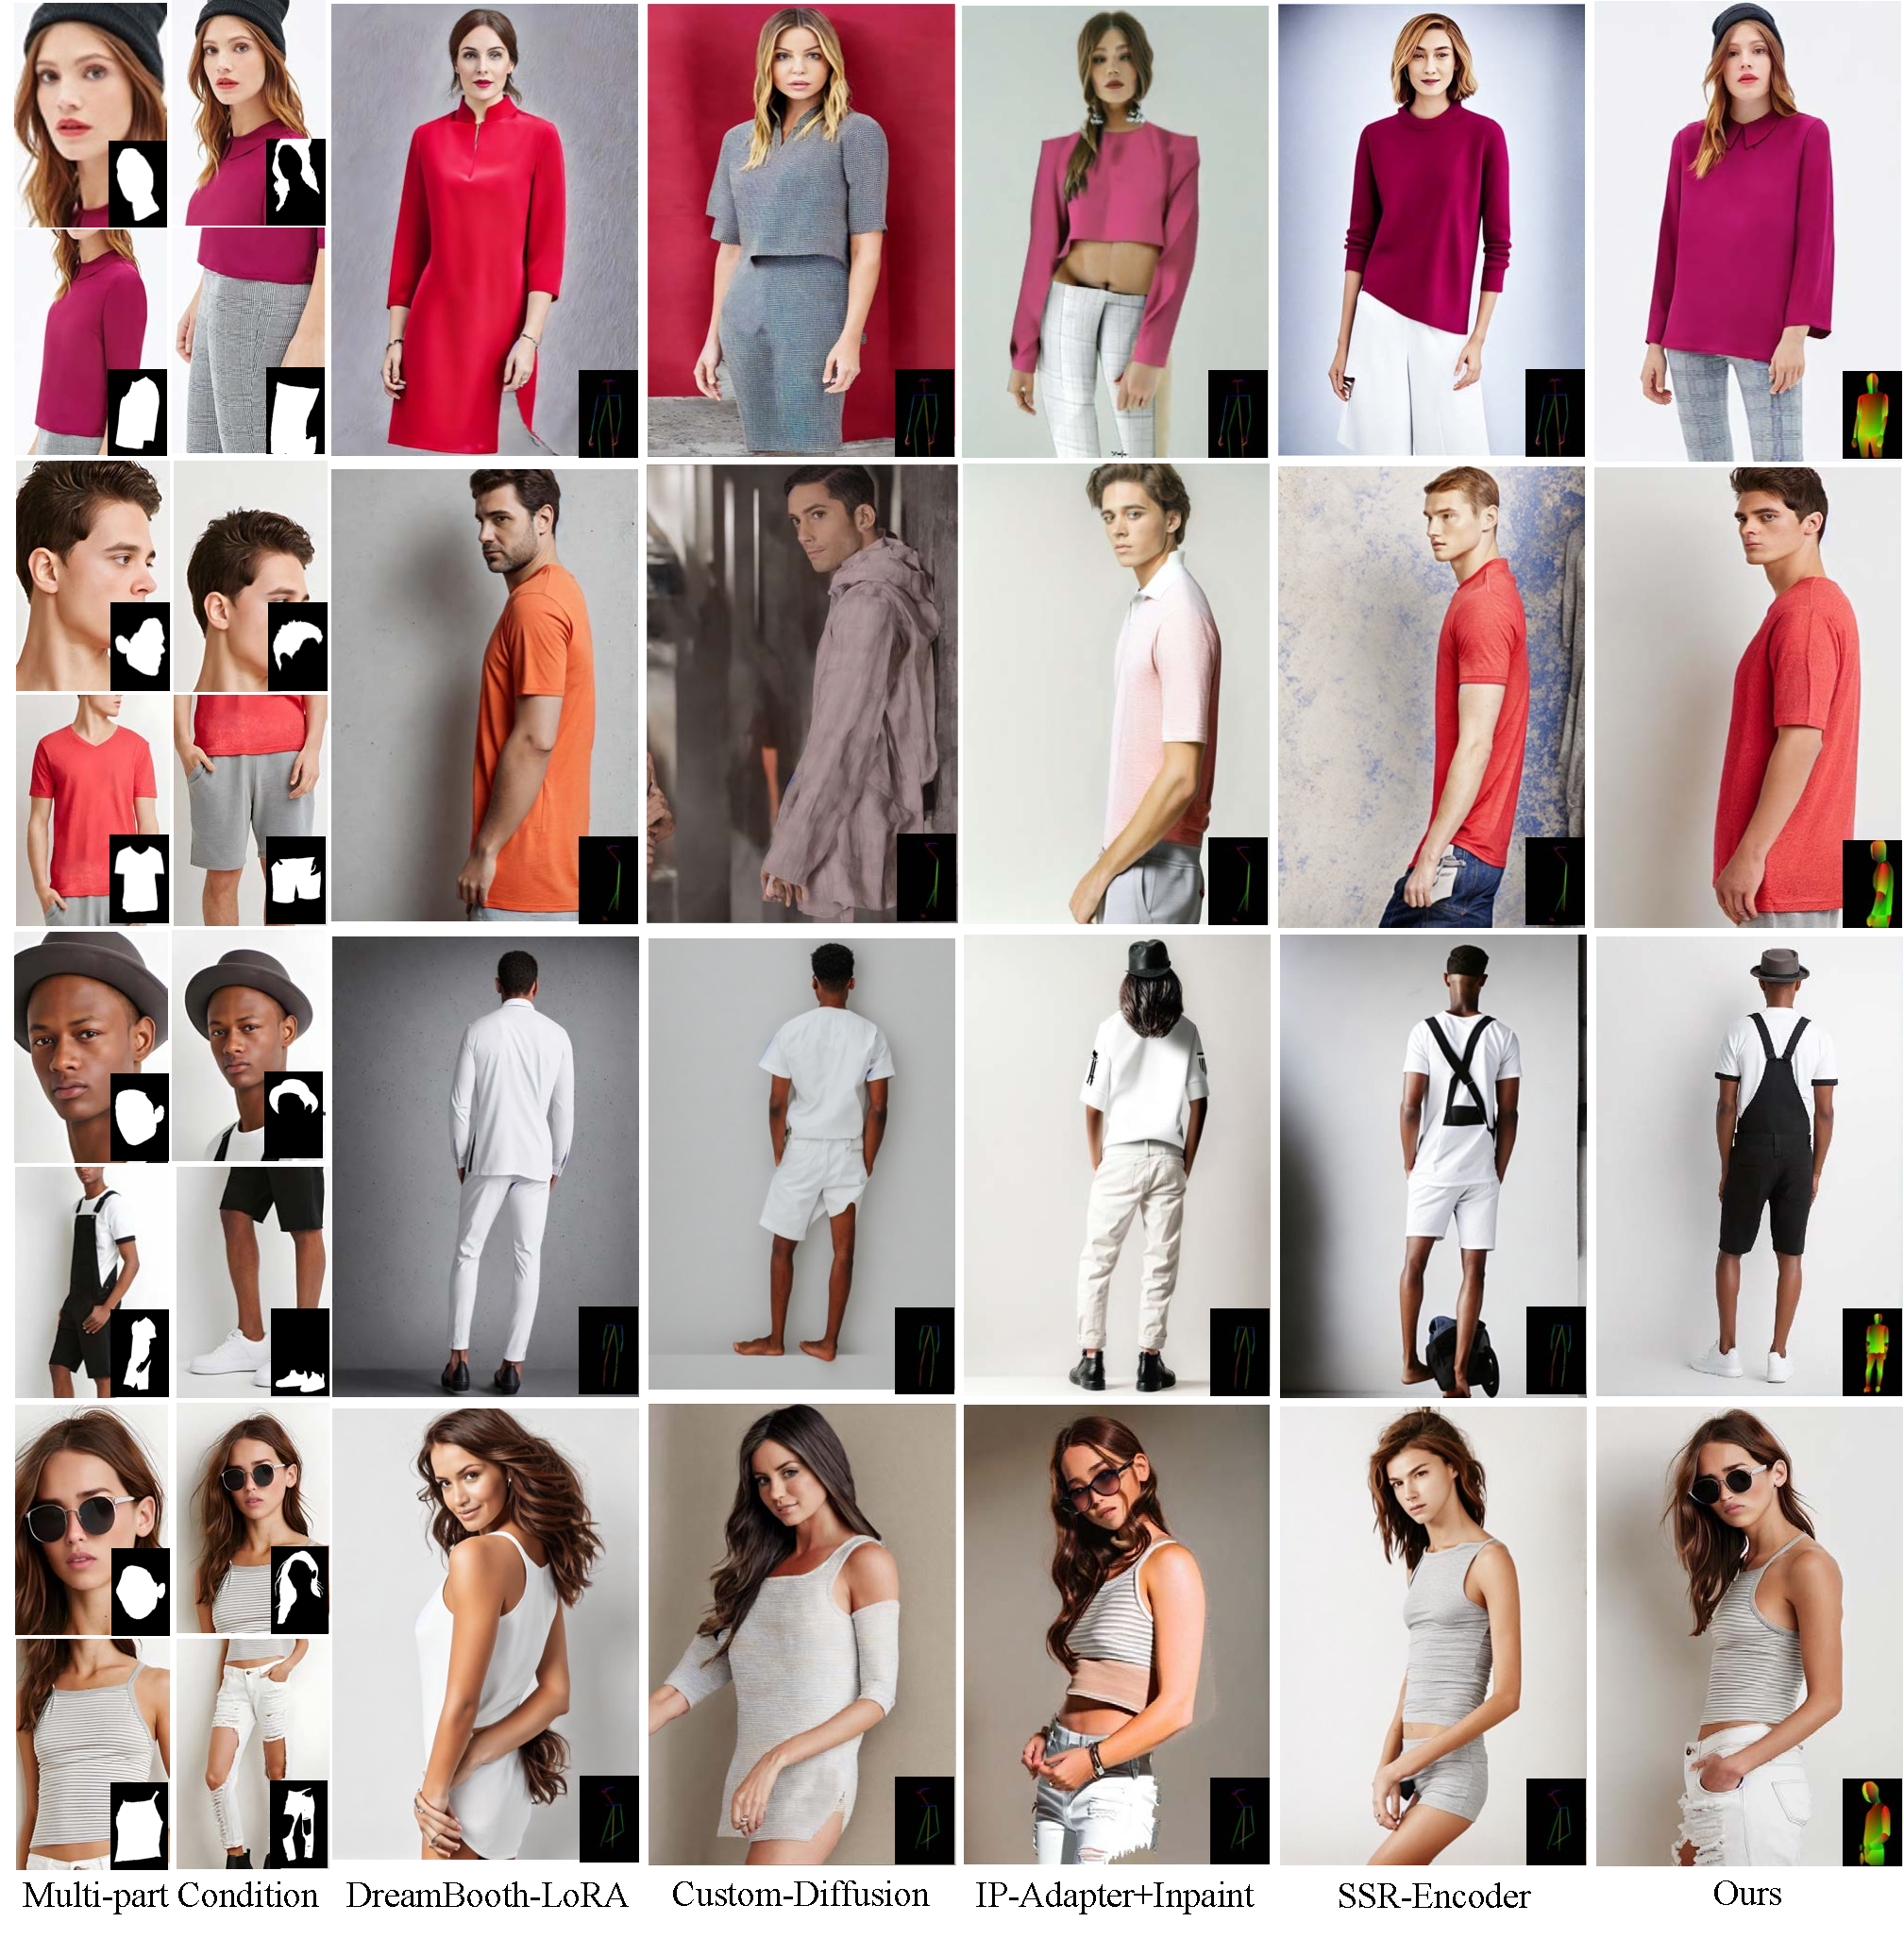
\includegraphics[width=\textwidth]{figure/comparison.pdf}
    \caption{Qualitative results generated by Parts2Whole and existing alternatives on our partitioned test set. We do not show the text condition in the figure, but notably, when we input the reference images to our proposed appearance encoder, we will pass in short labels such as face, hair or headwear, upper body clothes, lower body clothes, whole body clothes, shoes, etc.}
    \label{fig:comparison}
\end{figure*}

\subsection{Implementation Details}

\cparagraph{Dataset.}
To train the Parts2Whole model, we build a multi-modal dataset comprising about 41,500 reference-target pairs from the open-source DeepFashion-MultiModal dataset~\cite{jiang2022text2human,liuLQWTcvpr16DeepFashion}. 
Each pair in this newly constructed dataset includes multiple reference images, which encompass human pose images (e.g., OpenPose, Human Parsing, DensePose), various aspects of human appearance (e.g., hair, face, clothes, shoes) with their short textual labels, and a target image featuring the same individual (ID) in the same outfit but in a different pose, along with textual captions.

The DeepFashion-MultiModal dataset exhibits noise in its ID data. For example, different images are tagged with the same ID but depict different individuals. To address this issue, we first cleanse the IDs by extracting facial ID features from images tagged with the same ID using InsightFace\cite{deng2018arcface, InsightFaceProject}. Cosine similarity is then used to evaluate the similarity between image ID feature pairs to distinguish between different ID images within the same ID group. Subsequently, we utilize DWPose\cite{yang2023dwpose} to generate pose images corresponding to each image. Guided by human parsing files, we crop human images into various parts. Due to the low resolution of the cropped parts, we apply Real-ESRGAN\cite{wang2021realesrgan} to enhance the image resolution, thus obtaining clearer reference images. Textual descriptions of the original dataset are used as captions. For constructing pairs, we select images with cleaned IDs that feature the same clothes and individual but in different poses. Specifically, a pair contains multiple parts from one human image as reference images, and an image of the person in another pose as the target. Finally, we build a total of about 41,500 pairs, of which the training set is about 40,000 and the test set is about 1,500 pairs.

\cparagraph{Detailed Configurations.}
In this work, the denoising U-Net and the appearance encoder both leverage the pre-trained weights from Stable Diffusion-1.5~\cite{rombach2022ldm}. We use CLIP Vision Model with projection layers as our image encoder, initialized with Stable Diffusion Image Variations~\cite{sdimagevariation}. During training, we set the initial learning rate 1e-5 with a batch size of 64. The model is trained using 8 A800 GPUs, for a total of 30000 iterations. To maintain the capability of image generation, we randomly drop all of the reference image features and the pose condition with a probability of 0.2. At the same time, to improve the flexibility of generation, we randomly drop each appearance condition with a probability of 0.2, so that the human images can be generating from indefinite reference images. At the inference stage, we adopt DDIM sampler~\cite{song2020ddim} with 50 steps, and set the guidance scale to 7.5.

\subsection{Comparison with Existing Alternatives}

Our Parts2Whole targets at controllable human image generation conditioned on multiple parts of human appearance. To evaluate the performance of our proposed framework, we compare our Parts2Whole with existing subject-driven solutions. For fairness, we make some improvements to the methods, to make them more suitable for generating human images from multiple conditions.

\cparagraph{Test-time Fine-tuning Methods.}
Among the tuning-based methods, we adopt DreamBooth LoRA~\cite{ruiz2023dreambooth,hu2021lora} and Custom Diffusion~\cite{kumari2023customdiffusion} as baseline methods for comparison, as these methods are relatively robust and effective. DreamBooth LoRA inserts a smaller number of new weights into Stable Diffusion~\cite{rombach2022ldm} and only trains these parameters on just a few images of a subject or style, thereby associating a special word in the prompt with the example images. Custom Diffusion fine-tunes only key and value projection matrices in the cross-attention layers to customize text-to-image models. Given as input several aspects of human appearance, we use these two methods to fine-tune Stable Diffusion, such that it learns to bind identifiers with specific human parts. As shown in \cref{fig:comparison}, when it comes to multi-aspect composition, the attributes of different parts in images generated by these tuning-base methods mix together, resulting in unrealistic human images. In contrast, Parts2Whole generates high-fidelity results without the need for parameter tuning.

\cparagraph{Reference-based Methods.}
Among the tuning-free methods, we adopt IP-Adapter~\cite{ye2023ipadapter} and SSR-Encoder~\cite{zhang2024ssrencoder} for comparison. IP-Adapter is an image prompt adapter that can be plugged into diffusion models to enable image prompting, and can be combined with other adapters like ControlNet~\cite{zhang2023controlnet}. We firstly use IP-Adapter FaceID and ControlNet to generate human images from facial appearance and pose maps. Then we repaint hair, clothes, shoes and other areas using the specific image step by step, thereby achieving multi-image conditioned generation of portraits in a multi-step way. SSR-Encoder is an effective encoder designed for selectively capturing any subject from single or multiple reference images by the text query or mask query. For fairness, we fine-tune it in our human dataset to enhance its ability for human images.

We compare our Parts2Whole with the above two reference-based alternatives in the test set. For quantitative comparison, we compute the commonly used CLIP score and DINO score to evaluate the similarity between the generated image and the specified human parts. For further alignment evaluation, we use DreamSim~\cite{fu2023dreamsim}, a new metric for perceptual image similarity that bridges the gap between ``low-level'' metrics (e.g., LPIPS, PSNR, SSIM) and ``high-level'' measures (e.g., CLIP). Since the generated image is conditioned on multiple parts of human appearance, it is difficult to evaluate the degree of alignment by calculating the average metric with these multiple images. Therefore, we calculate the above three indicators between the output image and the original reference portrait from which these different parts come. We present the quantitative results in \cref{tab:quan_comp} and the qualitative results in ~\cref{fig:comparison}. Both IP-Adapter and SSR-Encoder fail to maintain alignment with the specified appearance images and often produce unrealistic results when multi-part combinations are involved. In comparison, our method achieves the best results in terms of image quality and appearance alignment.

\begin{table}\small
  \centering
  \caption{Quantitative comparison between our Parts2Whole and existing reference-based alternatives.}
  \begin{tabular}{@{}lccc@{}}
    \toprule
    Method & CLIP$\uparrow$ & DINO$\uparrow$ & DreamSim\cite{fu2023dreamsim}$\downarrow$ \\
    \midrule
    IP-Adapter~\cite{ye2023ipadapter} + Inpaint & 80.1 & 69.8 & 0.445   \\
    SSR-Encoder~\cite{zhang2024ssrencoder} & 86.9 & 75.1 & 0.346 \\
   Parts2Whole (Ours) & \textbf{91.2} & \textbf{93.7} & \textbf{0.221}  \\
    \bottomrule
  \end{tabular}
  \label{tab:quan_comp}
\end{table}

\cparagraph{User Study.}
We conduct a user study to further evaluate the reference-based methods IP-Adapter~\cite{ye2023ipadapter}, SSR-Encoder~\cite{zhang2024ssrencoder} and our Parts2Whole. We randomly select 20 pairs of reference-target pairs from the test set. For each pair, we provide multiple referential appearance images, pose images, textual captions, and the generated human images. We evaluate the performance from two main aspects: first, the \textbf{quality} of the generated images, which primarily refers to the realism, rationality, and clarity of the images; and second, the \textbf{similarity} between the generated images and the reference images. The similarity assessment includes consistency in ID, pose, texture, and color between the generated images and the reference images. We involve 20 users in the user study, who are required to score the three methods based on these two evaluative aspects. The final experimental results are shown in \cref{tab:user_study}, from which we observe that our model owns obvious superiorities for alignment with given appearance conditions.

\begin{table}
  \centering
  \caption{User study on the comparison with existing reference-based alternatives. ``Quality'' and ``Similarity'' measures synthesis quality and appearance preservation. Each metric is rated from 1 (worst) to 5 (best).}
  \begin{tabular}{@{}lcccc@{}}
    \toprule
    Method & Quality$\uparrow$ & Similarity$\uparrow$ \\
    \midrule
    IP-Adapter~\cite{ye2023ipadapter} + Inpaint &  3.78 & 3.58  \\
    SSR-Encoder~\cite{zhang2024ssrencoder} & 3.64  & 3.14 \\
   Parts2Whole (Ours) & \textbf{4.52} & \textbf{4.55} \\
    \bottomrule
  \end{tabular}
  \label{tab:user_study}
\end{table}

\subsection{Ablation Studies}

\begin{figure*}
    \centering
    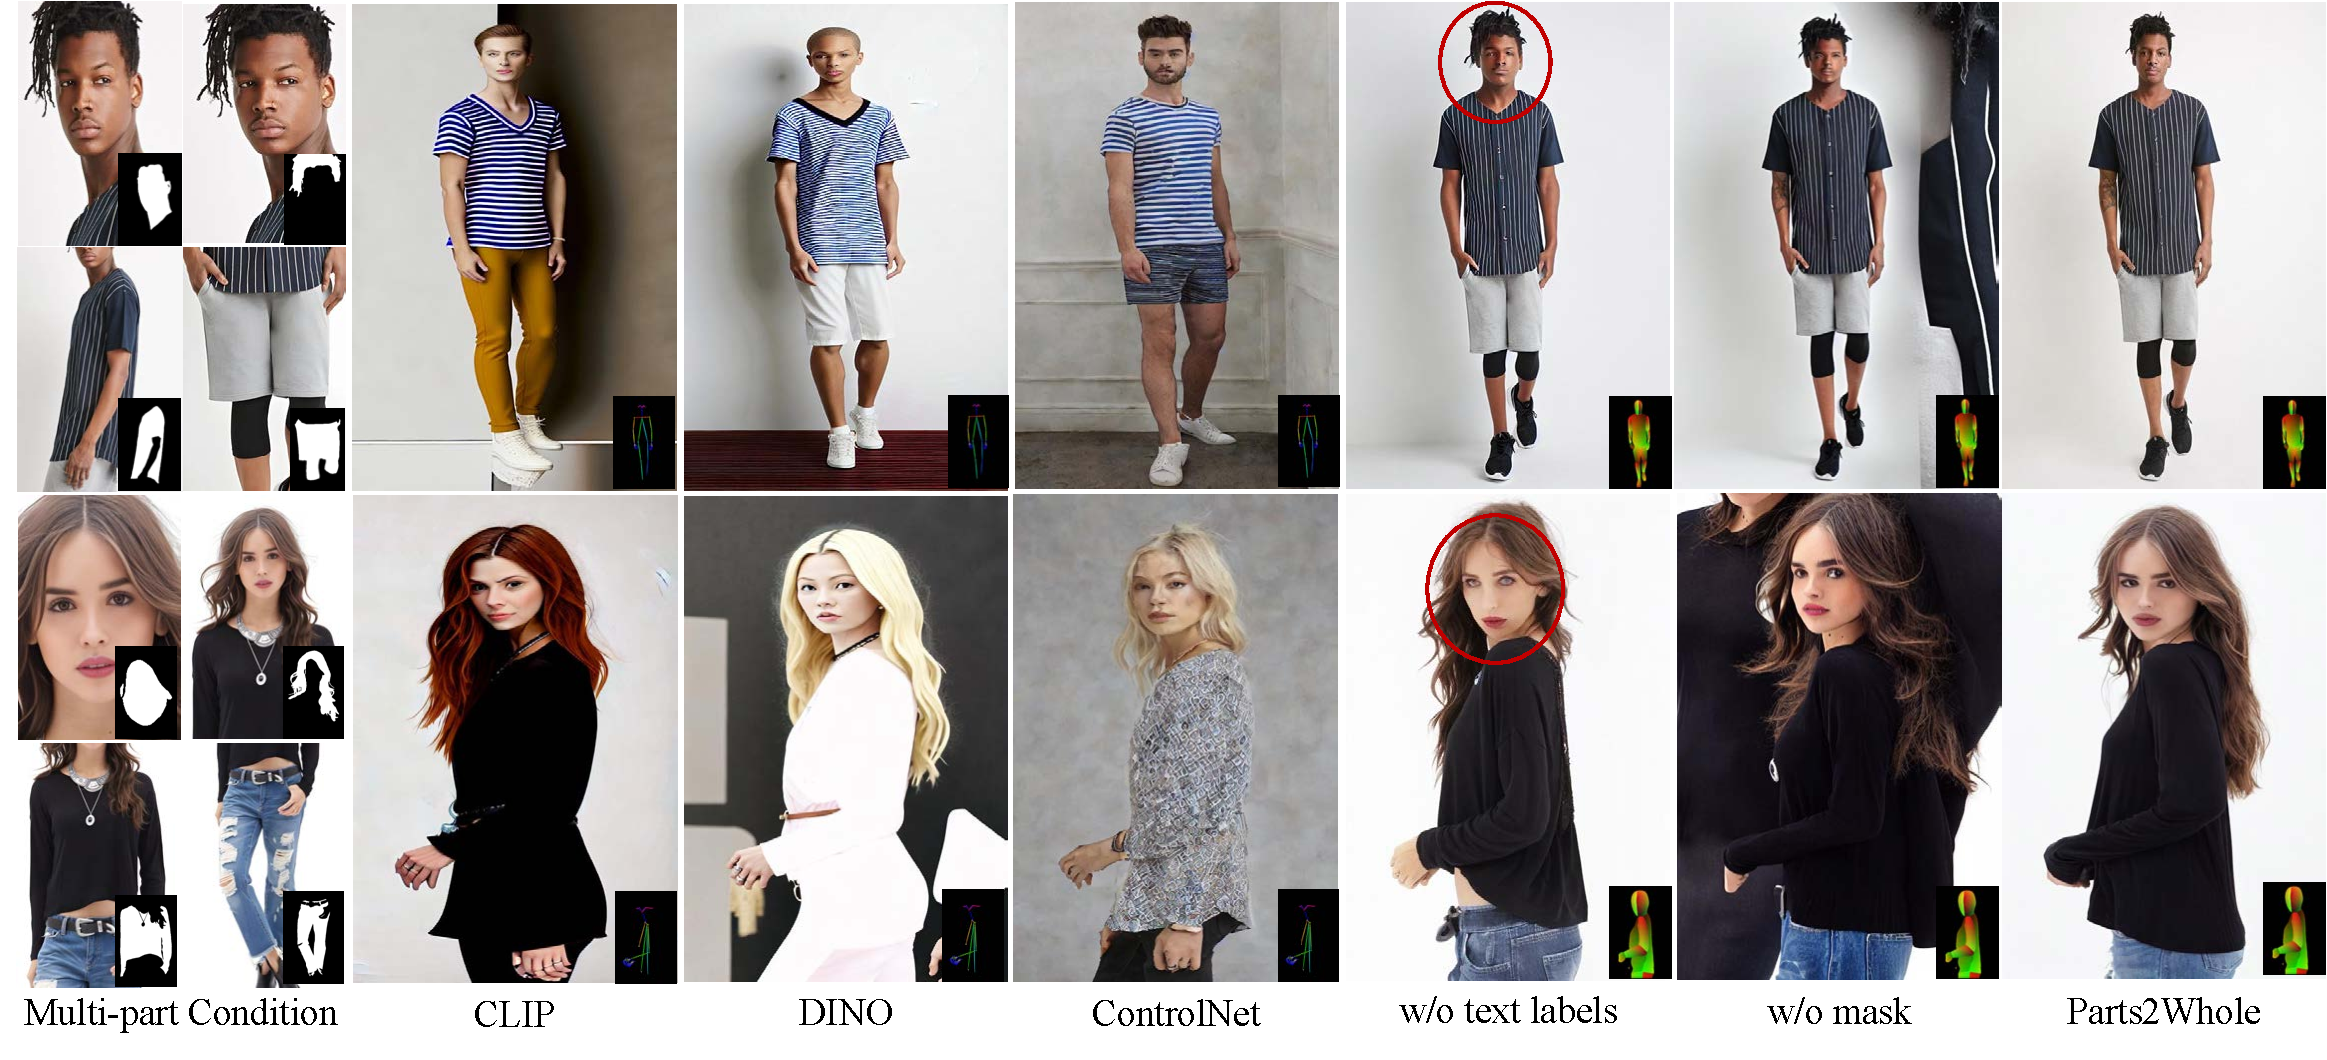
\includegraphics[width=\textwidth]{figure/ablation.pdf}
    \caption{Qualitative analysis of using different backbones for the appearance encoder, and our proposed methods.}
    \label{fig:ablation}
\end{figure*}

\cparagraph{Appearance Encoder for Multiple Images.}
As described in Sec.~\ref{subsec:unifiedref}, to extract detailed features from multiple reference images, our Parts2Whole designs an appearance encoder by copying the network structure and pre-trained weights from the denoising U-Net. Here, we compare it to the baseline with other image encoders. Specifically, we leverage the CLIP image encoder~\cite{radford2021clip}, DINOv2~\cite{oquab2024dinov2}, and ControlNet~\cite{zhang2023controlnet} as feature extractors and apply the same training settings for fair comparison. The qualitative results of generated human images are presented in \cref{fig:ablation}. From the second and third columns of the figure, we observe that these semantic-level feature extractors cannot preserve the appearance details of multiple reference images and only extract color and rough texture. ControlNet directly adds different image features with misaligned structures to the feature maps, resulting in unstable image quality. In contrast, our proposed appearance encoder provides fine-grained details of multiple aspects of human appearance.

\cparagraph{Semantic-Aware Encoder.} In the process of encoding multiple reference image features, we provide a textual class label for each aspect of human appearance, thus providing a classifier-like guidance. To assess the effectiveness of the additional external condition, we compare it with directly concatenating multiple reference images in the dimension of width as input to the appearance encoder. As shown in the 5th column in \cref{fig:ablation}, simply piecing reference images produces images relatively aligned with the given images, but leads to stiff-looking and unrealistic results. This is because modeling only the image itself makes the model lack awareness of different types of appearances. Conversely, after injecting different semantic labels for each reference image, the model has an awareness of various parts of the human appearance, producing realistic and flexible portraits.

\cparagraph{Mask-Guided Subject Selection.}
To precisely select subjects from multiple reference images, we introduce the subject masks into the shared self-attention mechanism. To evaluate the effectiveness of our proposed mask-guided attention, we compare it with that without masks. When not using subject masks, the image is generated with reference to all patches of the conditional images, including the unexpected background or other parts. As shown in \cref{fig:ablation}, due to the generation being interfered with by irrelevant subjects, the model produces homogeneous colors or appears with unexpected backgrounds or subjects. On the contrary, with the support of mask-guided attention, Parts2Whole accurately refers to the appearance of the specified parts to generate real human images.

\begin{table}\small
  \centering
  \caption{Quantitative analysis of using semantic-aware encoder and mask-guided subject selection.}
  \begin{tabular}{@{}lcccc@{}}
    \toprule
    Method & CLIP$\uparrow$ & DINO$\uparrow$ & DreamSim\cite{fu2023dreamsim}$\downarrow$ & FID$\downarrow$ \\
    \midrule
    w/o text labels & 90.1 & 91.9 & 0.248 & 23.95 \\
    w/o mask & 90.8 & 91.6 & 0.243 & 19.79 \\
   Parts2Whole & \textbf{91.2} & \textbf{93.7} & \textbf{0.221} & \textbf{17.29} \\
    \bottomrule
  \end{tabular}
  \label{tab:abla}
\end{table}

\begin{figure*}
    \centering
    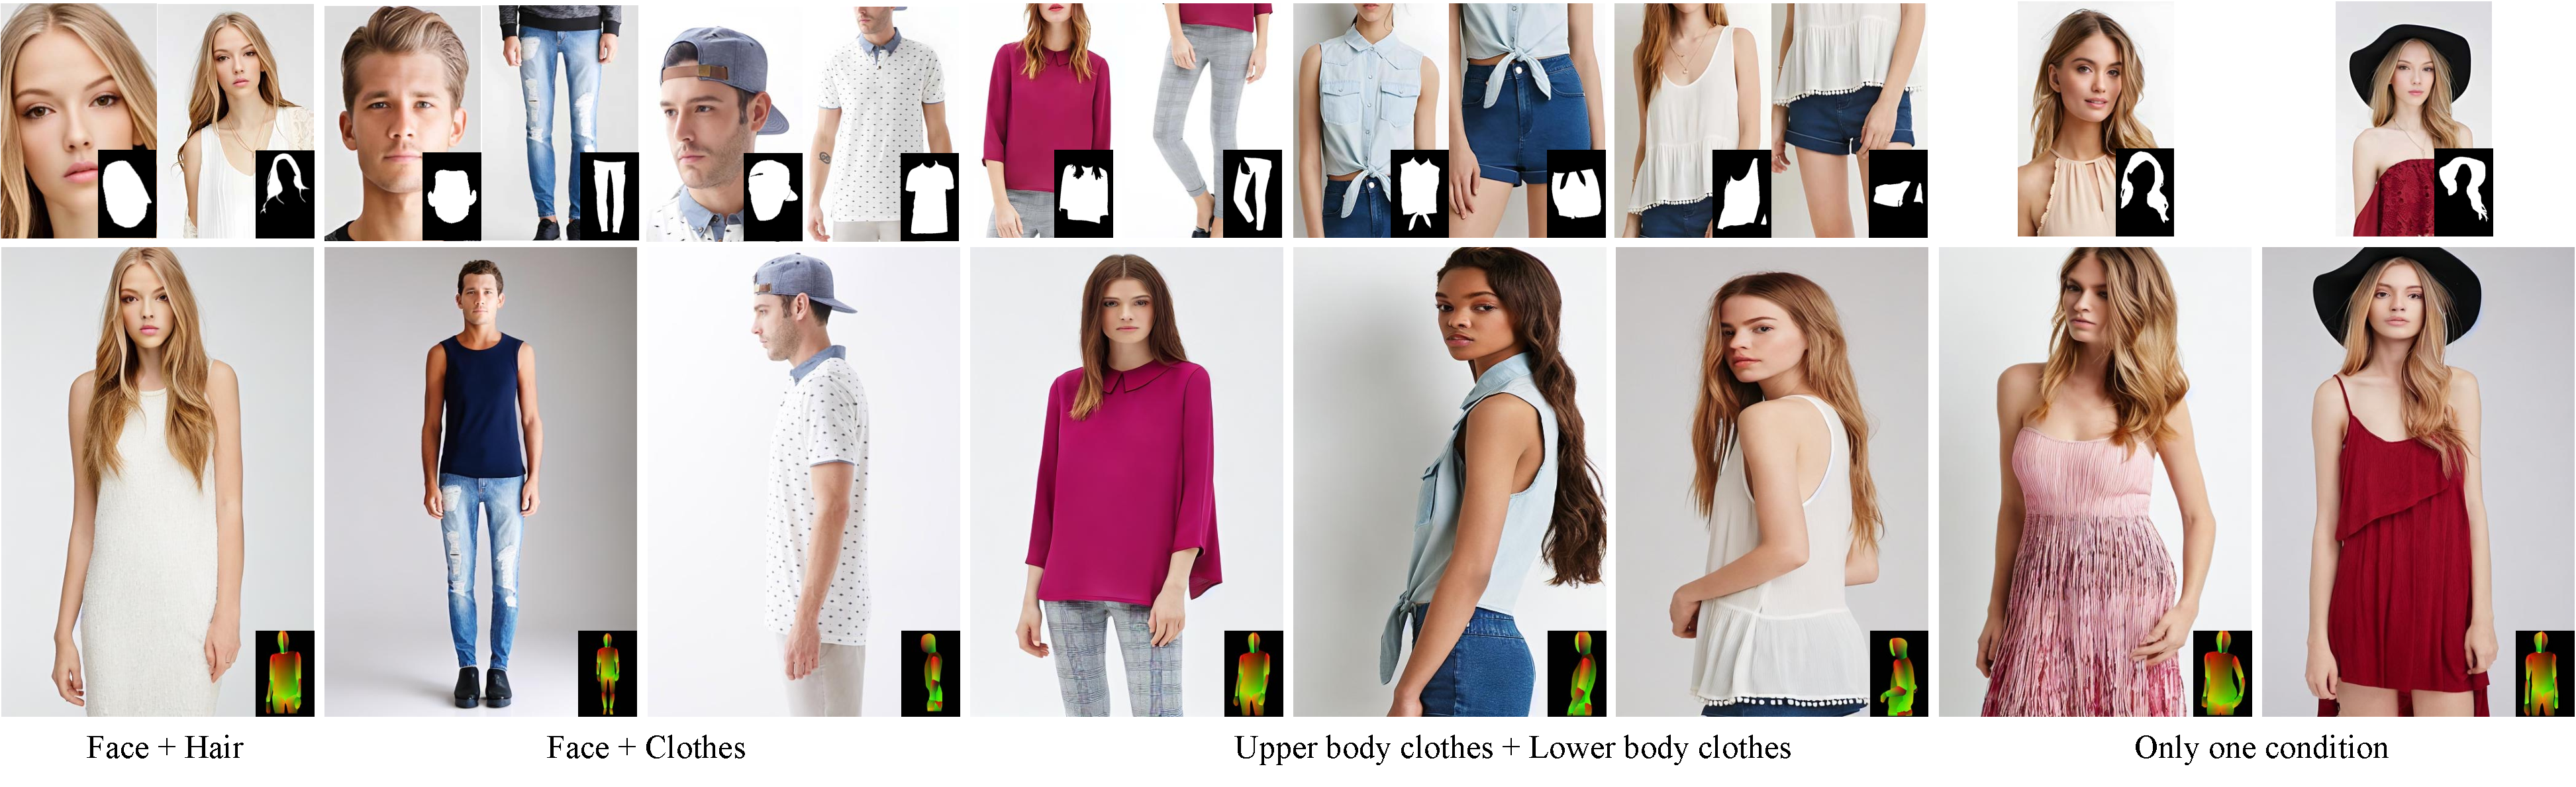
\includegraphics[width=\textwidth]{figure/any_quantity.pdf}
    \caption{The generated results from combinations of a different number of conditions.}
    \label{fig:any_quantity}
\end{figure*}

\subsection{More Results}
\begin{figure*}
    \centering
    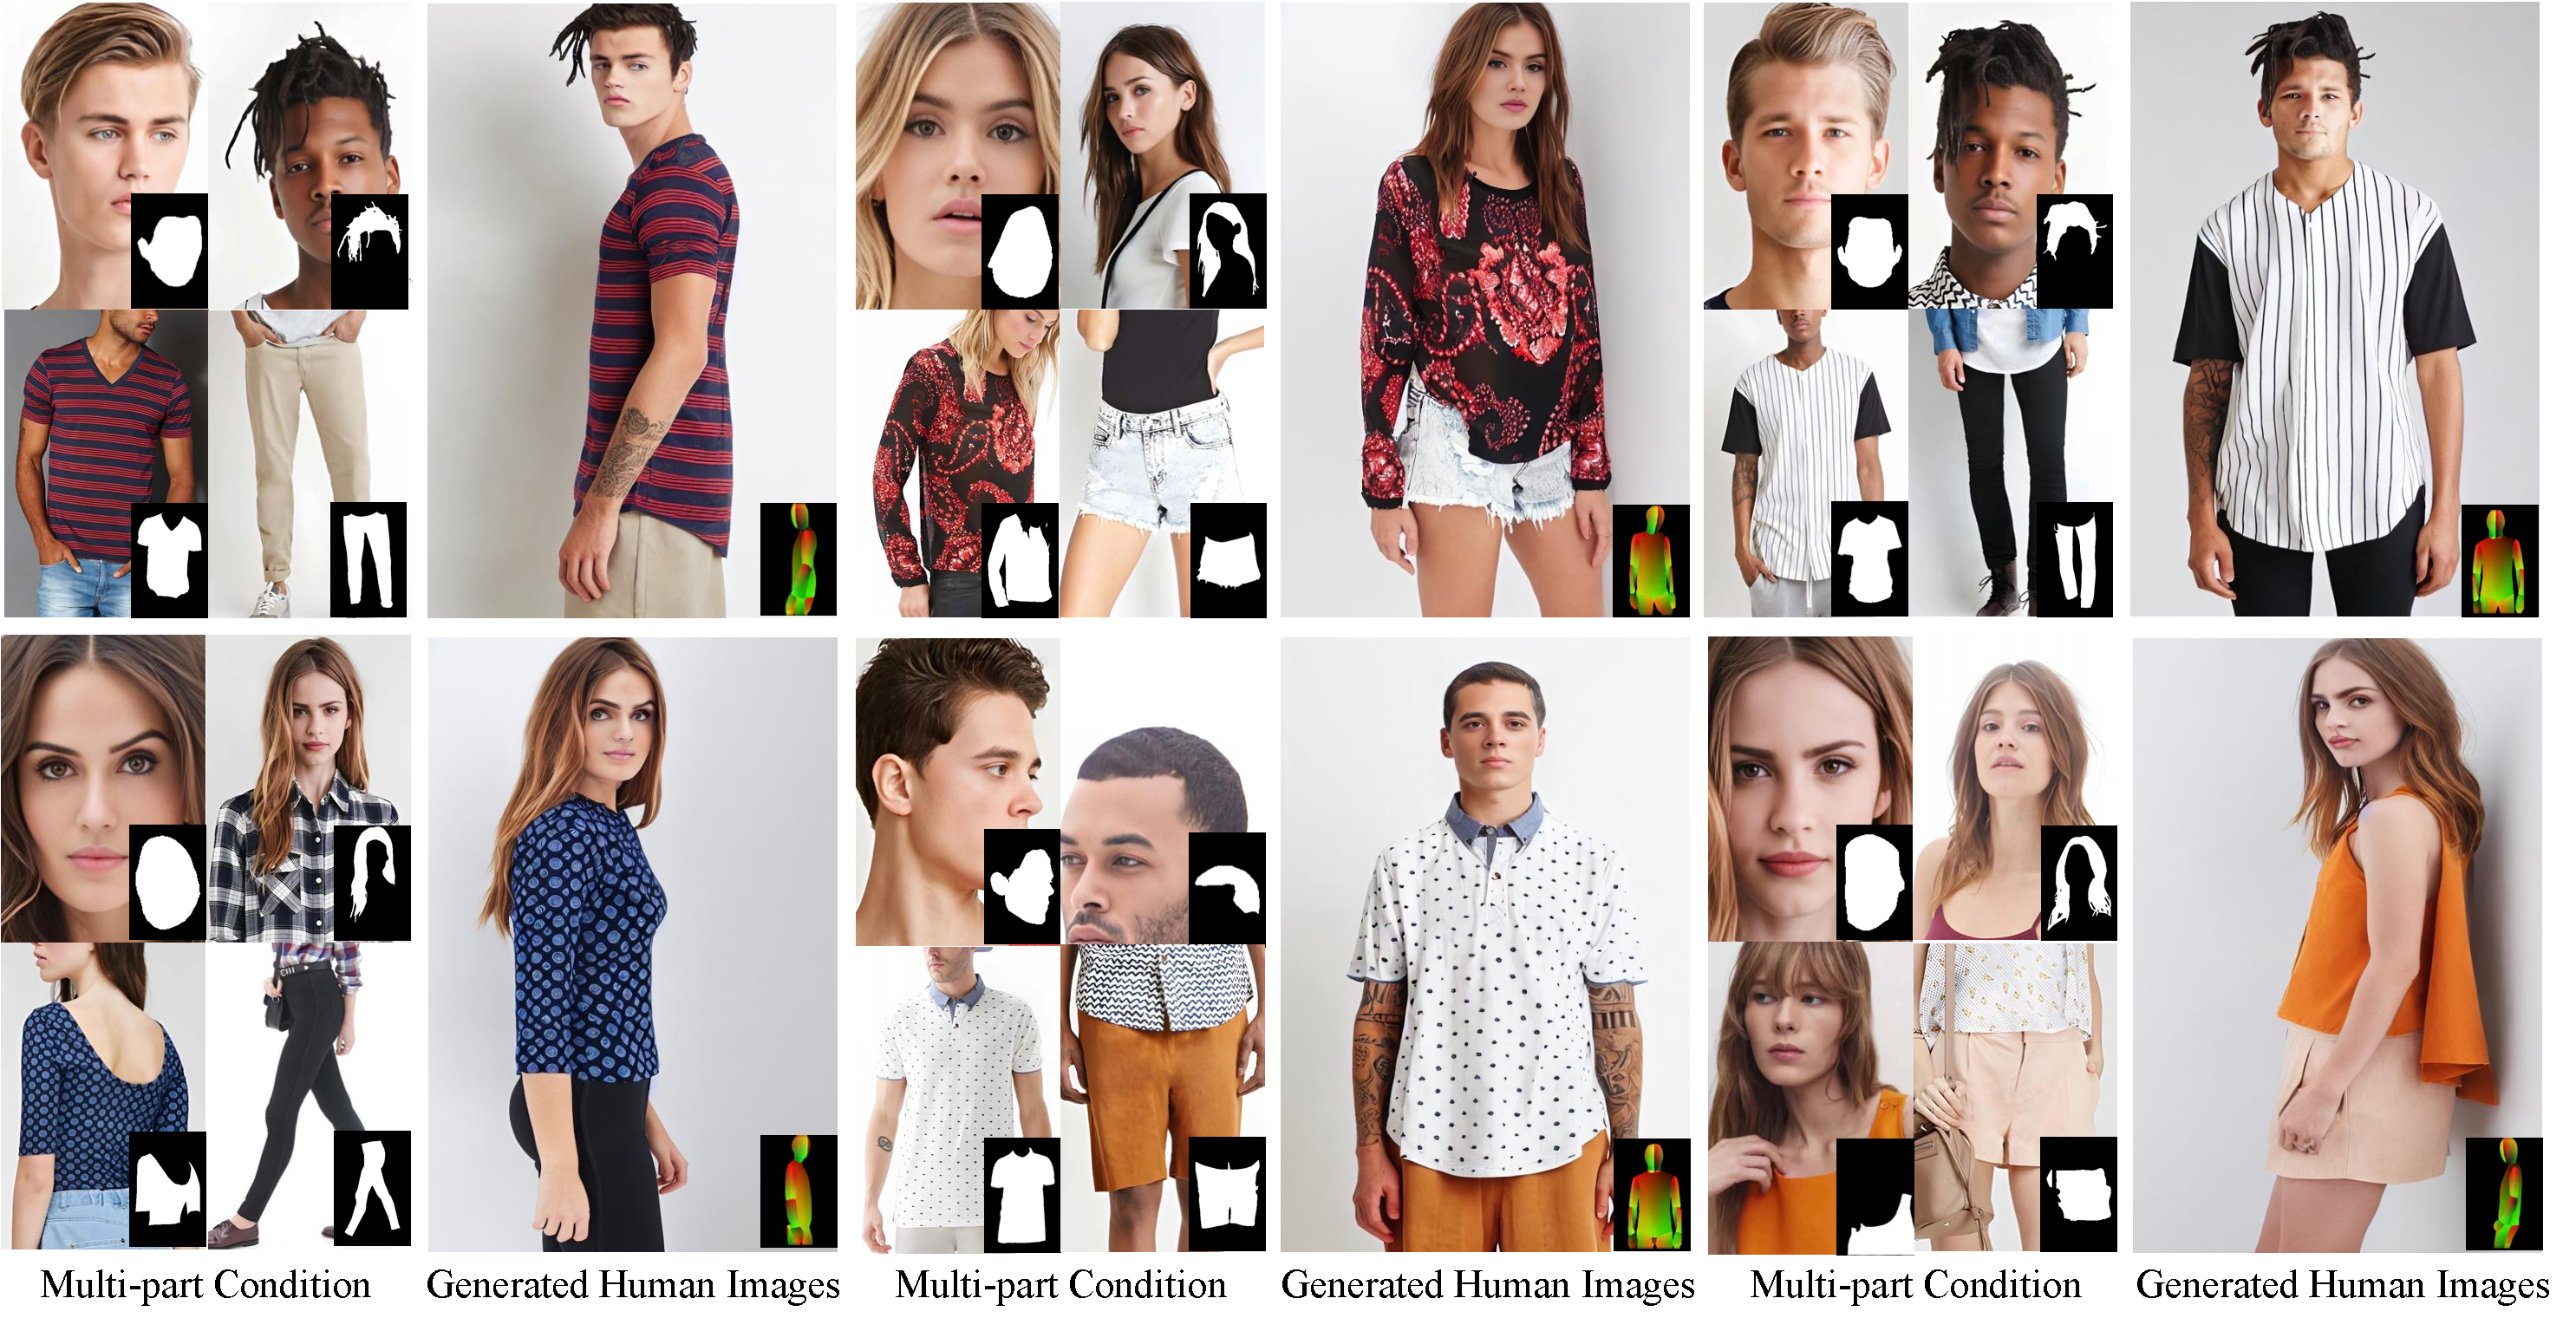
\includegraphics[width=\textwidth]{figure/any_person.pdf}
    \caption{Results of image generation using selected parts from different individuals as control conditions.}
    \label{fig:any_person}
\end{figure*}

\cparagraph{Body Parts of Any Quantity.}
Our Parts2Whole is able to generate human images from varying numbers of condition images, such as single hair or face input, or arbitrary combinations like ``Face + Hair'', ``Face + Clothes'', and ``Upper body clothes + Lower body clothes''. The experimental results are presented in \cref{fig:any_quantity}. The generated results under different control condition combinations still maintain high quality and realism. This flexibility enables our method to have broader application.

\cparagraph{Multiple Parts from Different Humans.}
We select various parts from different human images to serve as conditional images. For example, the face from person A, the hair or headwear from person B, the upper clothes from person C, and the lower clothes from person D. These parts are collectively used as control conditions for generation. The experimental results, as shown in \cref{fig:any_person}, demonstrate that our method not only accurately maps different parts of the reference image to the corresponding regions in the target image but also effectively preserves the details of the conditions, producing realistic images.

\section{Conclusion}

In this paper, we propose a pioneering approach to explore the source-free domain adaptation (SFDA) for video object detection (VOD). Specifically, we developed a novel SFDA method for a one-stage-based detector, YOLOV. The proposed STAR-MT technique significantly improves the performance of the video object detector in adverse image conditions without access to the target domain label or source domain data. Owing to its unsupervised nature, this work can be seamlessly applied to real-world scenarios requiring VOD models. The proposed method could serve as a baseline for future research in unsupervised domain adaptation for video object detection. 



{
    \small
    \bibliographystyle{ieeenat_fullname}
    \bibliography{arxiv}
}

% WARNING: do not forget to delete the supplementary pages from your submission 
\clearpage
\setcounter{page}{1}
\maketitlesupplementary


\section{Rationale}
\label{sec:rationale}
% 
Having the supplementary compiled together with the main paper means that:
% 
\begin{itemize}
\item The supplementary can back-reference sections of the main paper, for example, we can refer to \cref{sec:intro};
\item The main paper can forward reference sub-sections within the supplementary explicitly (e.g. referring to a particular experiment); 
\item When submitted to arXiv, the supplementary will already included at the end of the paper.
\end{itemize}
% 
To split the supplementary pages from the main paper, you can use \href{https://support.apple.com/en-ca/guide/preview/prvw11793/mac#:~:text=Delete%20a%20page%20from%20a,or%20choose%20Edit%20%3E%20Delete).}{Preview (on macOS)}, \href{https://www.adobe.com/acrobat/how-to/delete-pages-from-pdf.html#:~:text=Choose%20%E2%80%9CTools%E2%80%9D%20%3E%20%E2%80%9COrganize,or%20pages%20from%20the%20file.}{Adobe Acrobat} (on all OSs), as well as \href{https://superuser.com/questions/517986/is-it-possible-to-delete-some-pages-of-a-pdf-document}{command line tools}.

\end{document}
